\chapter{Introdução}

Simulação é a imitação, ao longo do tempo, da execução de um processo real ou de um sistema\cite{DESS-PH-2010}. Uma simulação baseia-se na abstração das características chaves do que se deseja simular, construindo assim um modelo que representa, da maneira mais fiel possível, o comportamento real deste processo ou sistema. A simulação pode ser usada para prever um comportamento quando o sistema real não pode ser comprometido, ou por estar inacessível, ou por ser considerado perigoso ou inaceitável comprometer este sistema. Também pode ser empregada quando deseja-se antever o comportamento de um sistema que ainda não foi desenvolvido, ou simplesmente não exista\cite{REALWORLD-2008}.

A utilização de computadores para avaliar um modelo representativo de um sistema real leva à chamada simulação computacional. A simulação computacional tem sido amplamente empregada em diversos ramos, como simulação de circuitos elétricos \cite{SPICE}, simulação eletromagnética \cite{OskooiRo10}, simulação metereológica \cite{WEATHER}, simulação de serviços \cite{SERVICES}, simulação de tráfego e trânsito \cite{TRAFFIC}, entre outros.

Em alguns casos, como na simulação do comportamento de circuitos eletromagnéticos e na simulação metereológica, o modelo é baseado em uma simulação numérica\cite{NUMERICAL}. Já em casos como a simulação de tráfego e da simulação de serviços, o modelo é baseado em eventos discretos, onde a operação do sistema é representada como uma sequência cronológica de eventos. Este trabalho aborda a simulação baseada em eventos discretos.

\section{Simulação}

A simulação é uma técnica que permite prever e visualizar o comportamento de sistemas reais a partir de modelos matemáticos. As aplicações da simulação abrangem diversos benefícios, tais como: a possibilidade de antever possíveis problemas ou comportamentos indesejáveis de um sistema, auxílio na tomada de decisão sem a necessidade de intervir no sistema real, facilidade na manipulação e alteração dos modelos, economia de recursos (físicos e financeiros) durante a tomada de decisões, dentre outros.

Para utilizar a simulação é necessário construir e analisar modelos que representam o sistema. Os modelos podem ser classificados de diferentes formas. Uma classificação pode ser considerada verificando a influência ou não de variáveis aleatórias no sistema. Os modelos que sofrem influência de variações aleatórias são denominados modelos estocásticos, enquanto os modelos que são livres de tal comportamento são denominados modelos determinísticos.

Os modelos que descrevem o comportamento através do tempo podem também ser classificados como contínuos ou discretos no tempo. Nos modelos de estados contínuos as variáveis de estados variam espontaneamente. Já nos modelos de estados discretos, as mudanças ocorrem em pontos específicos e descontínuos do tempo.

Este trabalho enfoca os modelos estocásticos e de estados discretos, uma vez que eles são os que melhor representam modelos de sistemas computacionais.

\subsection{Simulação Sequencial}

Um sistema de simulação sequencial, onde uma única máquina executa toda a simulação, pode ser retratado como uma fila de eventos aguardando para serem tratados. Cada evento possui o seu tempo de execução, como pode ser visto na figura~\ref{fig:simul}, que deve ser obedecido para garantir consistência do resultado.

Neste modelo sequencial, o sistema responsável pela simulação retira o próximo evento da fila de execução para tratá-lo. Ao fim do seu processamento, um próximo evento é retirado da fila, e isto se repete até o final de lista de eventos futuros. O tratamento de um evento pode ou não resultar em dados que influenciem num processamento futuro.

A simulação possui um relógio lógico interno que simboliza o tempo lógico da simulação. A cada avanço deste tempo discreto, o valor do seu relógio lógico é incrementado, e é verificado na lista de eventos futuros se existe um evento cujo tempo previsto para a execução é igual ao valor atual do relógio lógico. Caso haja um evento a ser executado naquele determinado momento, este evento é retirado da fila de eventos futuros e é processado pela simulação.

A atualização do relógio lógico sofre influência do evento a ser processado. Ou seja, dependendo do modelo simulado, um evento pode demorar mais ou menos tempo para ser processado. Esta variação é levada em conta quando se atualiza o relógio lógico da simulação ao final do processamento de cada evento.

\begin{figure}
  \centerline{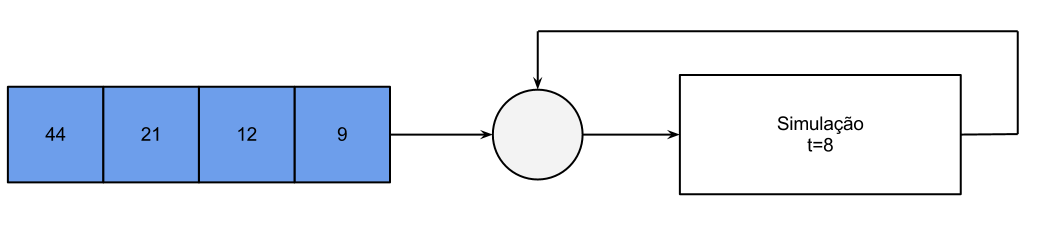
\includegraphics[scale=0.4]{simul_sequencial.png}}
  \caption{Simulação Sequencial.}
\label{fig:simul}
\end{figure}

Ainda dependendo do modelo a ser simulado, a execução de um evento pode resultar na criação de um novo evento que deve ser reinserido no sistema. Conforme ilustrado na figura~\ref{fig:simul_2}, ao se executar um evento no tempo $t=8$, um novo evento foi criado para ser processado no tempo $t=33$. Quando isso ocorre o evento é inserido na fila de eventos futuros, e aguarda para ser processado no tempo determinado.

Vale salientar que um processo nunca gera eventos para serem tratados em um tempo lógico inferior ao atual valor do seu relógio lógico interno. Ou seja, se o processo possui um tempo lógico $t=a$, um possível evento gerado em decorrência da execução de um evento neste determinado momento deverá ter um tempo $t=b$ de maneira que $b>a$.

\begin{figure}
  \centerline{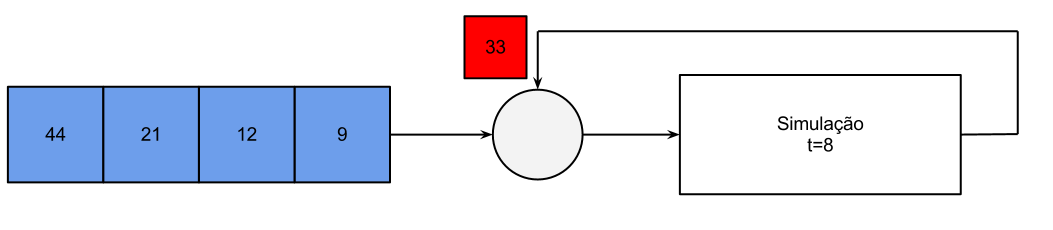
\includegraphics[scale=0.4]{simul_sequencial_2.png}}
  \caption{Geração de um novo evento.}
\label{fig:simul_2}
\end{figure}

\section{Simulação Distribuída}

A simulação é um processo que apresenta um alto custo computacional, devido a grande quantidade de dados que devem ser processados e a complexidade dos modelos matemáticos empregados. Esses fatores em conjunto podem encarecer computacionalmente o sistema, levando à ineficiência da simulação.

Uma das formas encontradas para se solucionar estes problemas foi dividir o tratamento dos diversos eventos entre vários processadores de uma mesma máquina paralela ou sobre um sistema distribuído, dando origem assim à Simulação Distribuída.

Distribuindo os eventos, reduz-se o tempo gasto pelos programas de simulação, mas, em contrapartida, novas situações necessitam de observação devido às características deste tipo de aplicação. É preciso sanar os problemas como a sincronização dos processos distribuídos, sobrecarga da rede de comunicação, necessidade de balanceamento de carga do sistema, dentre outros.

\section{Objetivo}

Conforme descrito, um dos problemas de se distribuir a simulação entre diversos nós de um sistema é a possibilidade de que os processos lógicos não sejam homogeneamente distribuídos, causando um desbalanceamento de carga no sistema. Isto pode ocorrer quando, por exemplo, processos que demandam um processamento mais intenso são agrupados em um mesmo nó, enquanto processos que não demandam tanto processamento são distribuídos pelo sistema. A concentração de processos com alta demanda de processamento em um mesmo nó do sistema levaria à sobrecarga deste nó, causando um desbalanceamento do sistema.

Outra situação que levaria a um desbalanceamento de carga é a existência de processos que se comunicam com uma frequência muito grande executando em nós distintos do sistemas, sobrecarregando a rede com troca de mensagens. Se fosse possível detectar os processos que se comunicam com maior frequência e agrupá-los em um mesmo nó do sistema, diminuiria-se consideravelmente o tráfego de mensagens na rede, aumentando o desempenho da simulação.

Para que seja feita a partição dos processos lógicos por entre os nós do sistemas existem algorítmos capazes de analisar o sistema, considerando fatores como volume de troca de mensagem e necessidade de processamento de cada processo lógico e mapear cada processo para um determinado nó do sistema.

Porém, para que isso seja possível, o processo lógico deve ser capaz de efetuar uma migraçõa, ou seja, deve ser capaz de interromper sua execução em um determinado instante, migrar para um nó diferente do sistema e, de maneira transparente, retornar à execução no ponto que ela foi interrompida.

O objetivo deste trabalho é a criação de um \textit{middleware} de comunicação que possibilite à um processo lógico efetuar de maneira transparente uma migração de um ambiente de simulação para outro. Este \textit{middleware} deve prover diversas facilidades além da mobilidade do processo lógico, como troca de mensagens entre os processos lógicos, redirecionamento de mensagens transientes (caso o processo tenha migrado no mesmo momento em que recebia uma mensagem), localização de um processo através de um endereço lógico que seja único em toda a simulação (mesmo o processo migrando para outro nó do sistema, deve ser possível comunicar com este processo usando apenas o seu endereço lógico) e serialização do processo lógico, necessário para se salvar o estado de um processo em um determinado momento.

Para validar o funcionamento do \textit{middleware} proposto foi desenvolvido também um micro-\textit{framework} utilizando este \textit{middleware} como base para todo o seu desenvolvimento.

\section{Organização do Documento}

O capítulo seguinte traz uma abordagem introdutória à simulação distribuída de eventos discretos e descreve o funcionamento de dois protocolos utilizados para sincronização de simulação distribuída.

O terceiro capítulo aprofunda-se na proposta do projeto, apresentando a arquitetura básica do \textit{middleware} de comunicação que visa proporcionar mobilidade aos processos lógicos no sistema de simulação distribuída. 

Os capítulos quatro e cinco apresentam, consecutivamente, a arquitetura interna do \textit{middleware} de comunicação e a arquitetura de um micro-\textit{framework} desenvolvido para demonstrar o funcionamento do \textit{middleware} de comunicação.

Por fim o capítulo seis traz alguns detalhes de implementação do \textit{middleware} proposto que o autor julgou conveniente descrever, seguido pela conclusão, compondo o sétimo capítulo.
